\section{Primer on programmable switches}
\label{s:architecture}

\begin{figure*}[t]
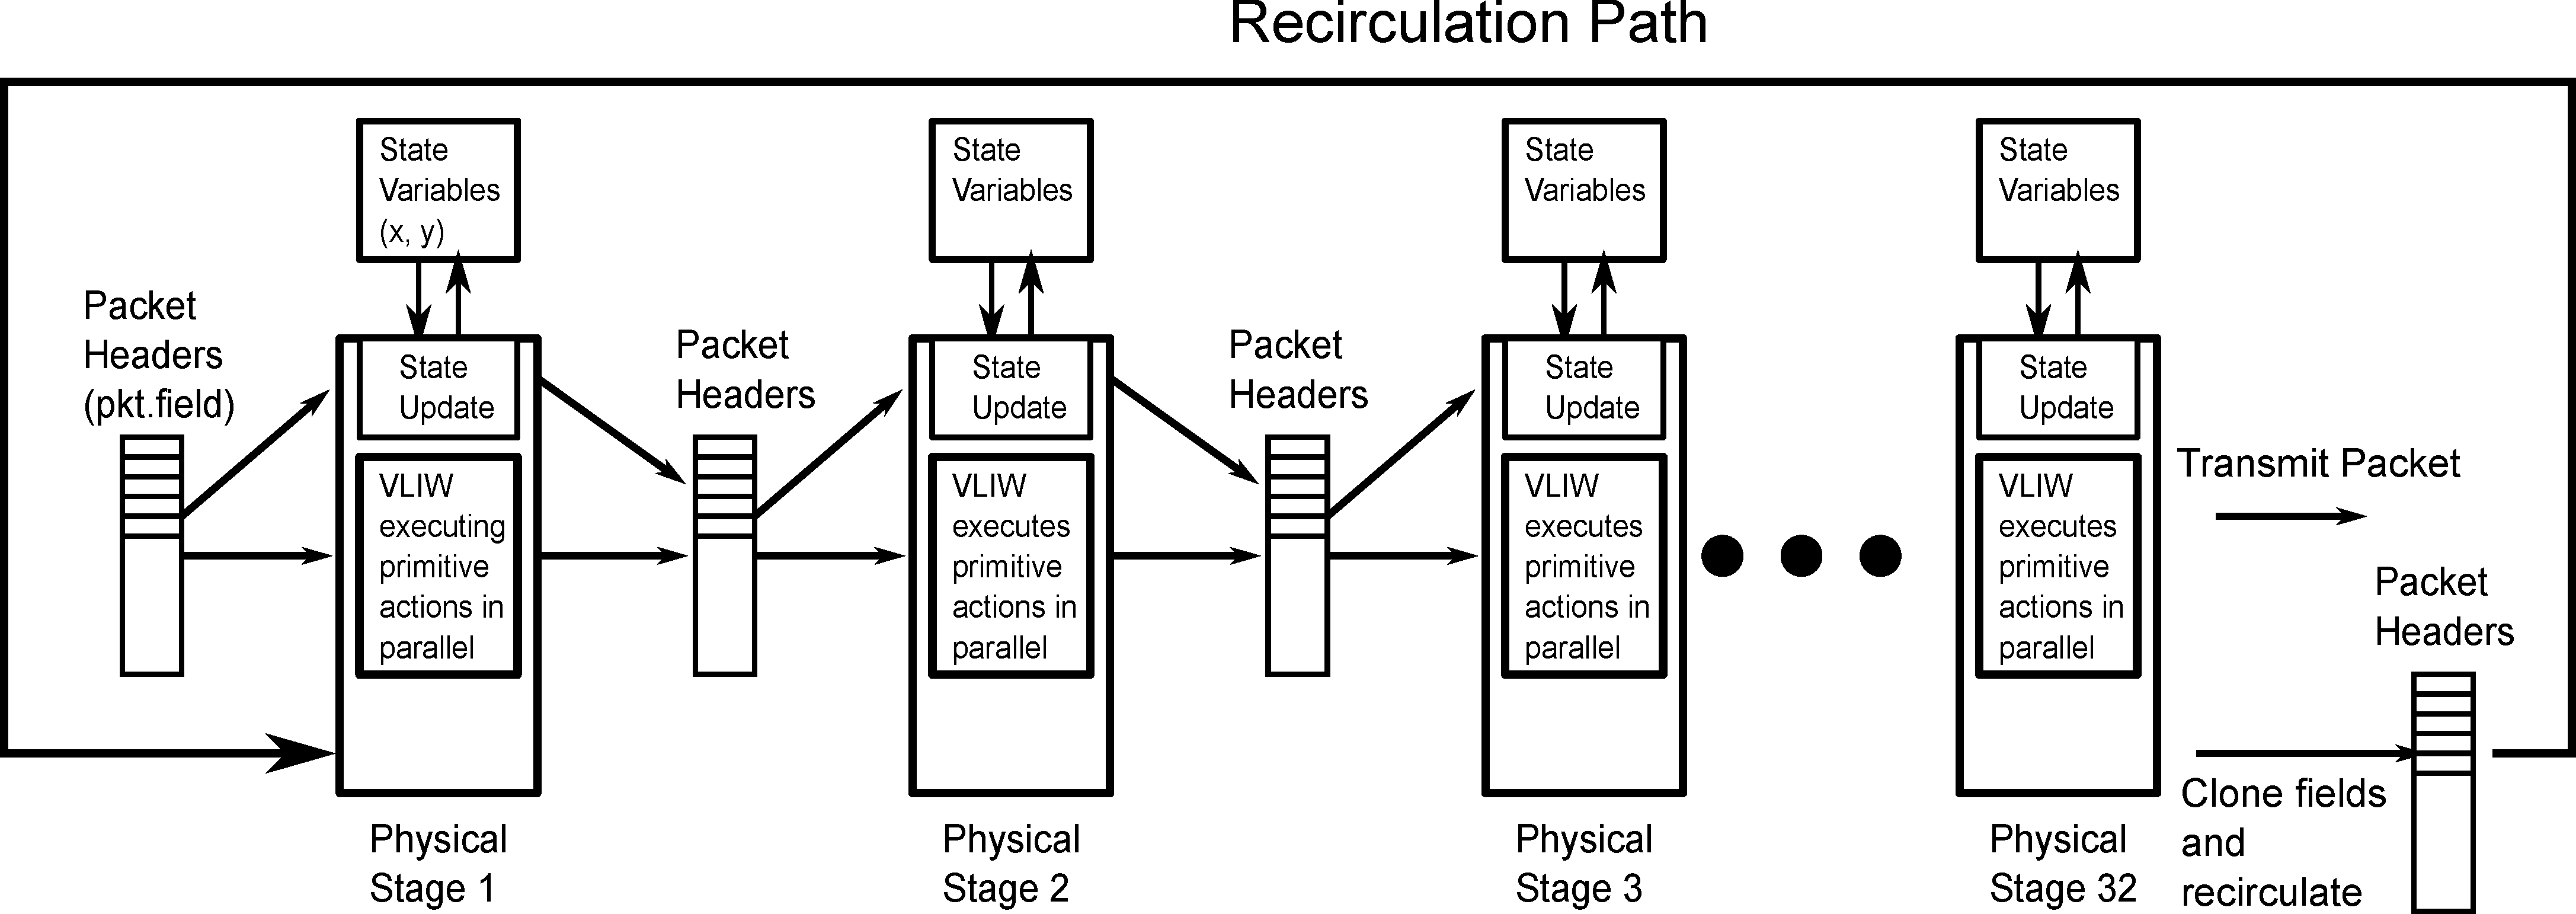
\includegraphics[width=\textwidth]{p4_switch_model.pdf}
\caption{The RMT architecture. Packet field and state variables correspond to
names used in Table~\ref{table:stateful_inst}}
\label{fig:architecture}
\end{figure*}

This section provides a brief primer on the architecture of a programmable
switch to provide sufficient context for the rest of the paper. For
concreteness, we describe the Reconfigurable Match-Action Table (RMT)
architecture~\cite{rmt}, a representative programmable switch architecture
targeted by \pktlanguage{}. Other switches with similar programmable
architectures include Intel's FlexPipe~\cite{flexpipe} and Cavium's
Xpliant~\cite{xpliant}.

Packets entering a programmable switch are parsed by a programmable parser that
turns packets into a set of header fields. The set of packet headers is first
processed by an ingress pipeline consisting of match-action tables arranged in
stages. The packet then enters the switch scheduler, and once it has exited the
scheduler, it is processed by a similar egress pipeline.

Packet processing itself happens within the match-action tables contained
inside these pipelines. Specifically, the actions carry out packet processing
in response to a match. Our discussion below focuses on the acitons executed
within each pipeline assuming some match-action table has been setup within
each pipeline stage to match on packets on interest.

{\textbf Actions within the pipeline}
The action unit within each pipeline stage~\ref{fig:architecture} processes
packet headers by applying a sequence of modifications to packet fields and/or
state stored in each stage. Each stage can carry out simple stateless
arithmetic operations (add/sub/shift) on packet fields using a Very Large
Instruction Word that carries out operations on distinct header fields in
parallel.

Each stage can also update state contained within that stage alone based both
on the previous value of the same state and packet header fields. This stateful
update is atomic: the updated value of state is available for the next packet.
However, it is very limited. Table~\ref{table:stateful_inst} illustrates a
sample of these stateful update instructions.

\begin{table}
\begin{small}
\begin{tabular}{|c|c|}
\hline
Instruction description & Form \\
\hline
Read and write & \texttt{x = pkt.field;} or \texttt{pkt.field = x;} \\
\hline
Read, modify, and write & \texttt{x = x + pkt.field;} \\
\hline
Conditional execution & \texttt{x = pkt.predicate ? pkt.field : x;} \\
\hline
\end{tabular}
\end{small}
\caption{Atomic stateful instructions in the RMT architecture. We use the
symbols {\tt x} to refer to stateful variables and {\tt pkt.<>} to refer to a
packet field. Both packet fields and stateful variables are also illustrated in
Figure~\ref{fig:architecture}}

\label{t:stateful_inst}
\end{table}
%\item Packed operations on pairs of stateful variables: \texttt{ (x, y) = (x + y, x - y);}
%\item Multiply and accumulate a stateful variable: \texttt{ x = x * pkt.field + pkt.field2; }

RMT is a shared-nothing architecture: state variables are local to a particular
stage in the ingress or egress pipeline and cannot be shared across pipeline
stages or pipelines. The RMT pipeline allows a stage to communicate state
information to a successor stage downstream by writing state into a packet
field. To let a stage communicate state information to a predecessor stage
upstream, the RMT architecture allows packets to be cloned and recirculated
back into a pipeline.

This way, a state variable $x$ can be read in stage 1, written downstream in stage
2, and then a cloned packet to stage 1 could update the state variable $x$ in stage 1.
However, recirculation has a cost: recirculated packets consume pipeline
capacity by taking away capacity from new data packets. Further, recirculation
latency can be large: several hundred packets might pass through the pipeline
before the recirculated packet updates state in stage 1.
